\documentclass[aspectratio=169,11pt]{beamer}

\usetheme{Madrid}
\usecolortheme{default}
\usepackage[utf8]{inputenc}
\usepackage[T1]{fontenc}
\usepackage[brazilian]{babel}
\usepackage{graphicx}
\usepackage{booktabs}
\usepackage{amsmath}
\usepackage{amssymb}

\definecolor{ufrjblue}{RGB}{0,74,128}
\setbeamercolor{structure}{fg=ufrjblue}
\setbeamercolor{title}{fg=white,bg=ufrjblue}
\setbeamercolor{frametitle}{fg=white,bg=ufrjblue}

\setbeamerfont{footnote}{size=\tiny}

\title{Explicando Decis\~oes de LLMs\\via Otimiza\c{c}\~ao Inversa}
\subtitle{Resultados Experimentais --- Execu\c{c}\~ao 29/03/2026}
\author{George Silva}
\date{Mar\c{c}o 2026}

\begin{document}

% ============================================================
\begin{frame}
\titlepage
\end{frame}

% ============================================================
\begin{frame}{Vis\~ao Geral da Pesquisa}
\textbf{Pergunta central:} LLMs possuem um processo de decis\~ao \textbf{est\'avel e aprend\'ivel}?

\vspace{0.3cm}
\textbf{Abordagem:} Otimiza\c{c}\~ao inversa --- inferir a fun\c{c}\~ao objetivo impl\'icita do LLM a partir de suas classifica\c{c}\~oes observadas.

\vspace{0.3cm}
\textbf{Modelo:} GPT-4o-mini (temperatura 0.0) \quad | \quad \textbf{Seeds:} 42, 123, 7, 256, 999

\vspace{0.3cm}
\textbf{Hip\'oteses:}
\begin{enumerate}
    \item[\textbf{H1}] O LLM mant\'em crit\'erio decis\'orio consistente (Kappa $> 0.7$)
    \item[\textbf{H2}] Few-shot amplifica a consist\^encia LLM--m\'etrica
    \item[\textbf{H3}] O LLM consegue aprender o crit\'erio de um perito externo
    \item[\textbf{H4}] Exemplos ``hard'' (pr\'oximos \`a fronteira) s\~ao mais informativos
    \item[\textbf{H5}] Comportamento \'e reproduz\'ivel entre execu\c{c}\~oes (5 seeds)
\end{enumerate}
\end{frame}

% ============================================================
\begin{frame}{Metodologia: Fases Experimentais}
\begin{columns}[T]
\begin{column}{0.48\textwidth}
\textbf{Fases A--C: M\'etrica Impl\'icita do LLM}
\begin{itemize}
    \item \textbf{Fase A:} LLM classifica 150 pontos 2D (zero-shot). Aprende-se $\hat{W}_{LLM}$ via Perceptron Estruturado / NNLS
    \item \textbf{Fase B:} Testa $\hat{W}_{LLM}$ em problema com centr\'oides deslocados
    \item \textbf{Fase C:} Testa $\hat{W}_{LLM}$ com distor\c{c}\~ao geom\'etrica maior
\end{itemize}
\end{column}
\begin{column}{0.48\textwidth}
\textbf{Fase D: LLM como Aprendiz}
\begin{itemize}
    \item Expert com m\'etrica $W$ conhecida rotula dados
    \item LLM recebe exemplos few-shot e deve reproduzir
    \item 4 estrat\'egias: easy, hard, mixed, random
    \item 3 experts: $W$=[0.3,1.5], [1.5,0.3], [1.0,1.0]
\end{itemize}

\vspace{0.3cm}
\textbf{Experimentos Adicionais:}
\begin{itemize}
    \item Vi\'es de nomes/ordem de classes
    \item Dilui\c{c}\~ao (hard + easy progressivos)
    \item Proje\c{c}\~ao R3 ($x_3 = x_1 \cdot x_2$)
    \item Compara\c{c}\~ao Perceptron vs.\ NNLS
\end{itemize}
\end{column}
\end{columns}
\end{frame}

% ============================================================
\begin{frame}{Dados Sint\'eticos: Problemas A, B e C}
\begin{center}
    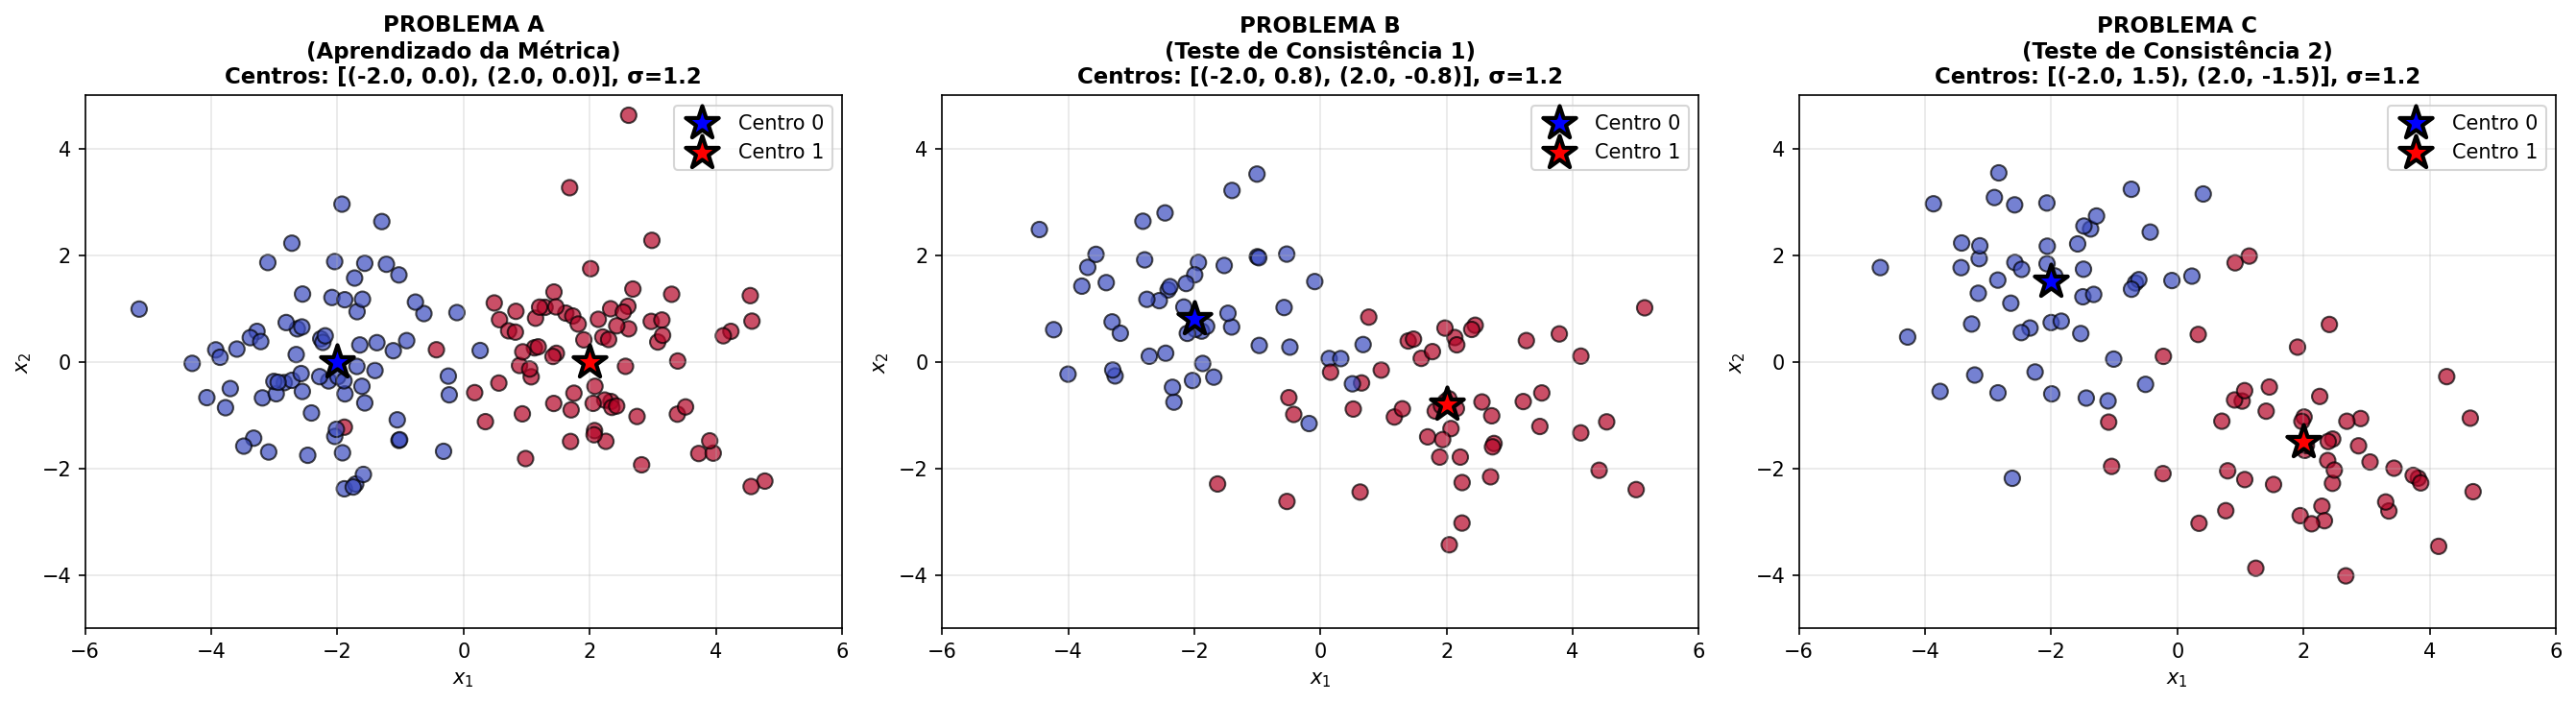
\includegraphics[width=0.85\textwidth]{01_all_three_problems.png}
\end{center}
\vspace{-0.2cm}
\small Tr\^es problemas 2D com Gaussianas. Problema A: refer\^encia (150 amostras). Problemas B e C: geometrias diferentes (100 amostras cada) para testar transfer\^encia da m\'etrica.
\end{frame}

% ============================================================
\begin{frame}{Fase A: Distribui\c{c}\~ao de $\hat{W}_{LLM}$ entre Seeds}
\begin{center}
    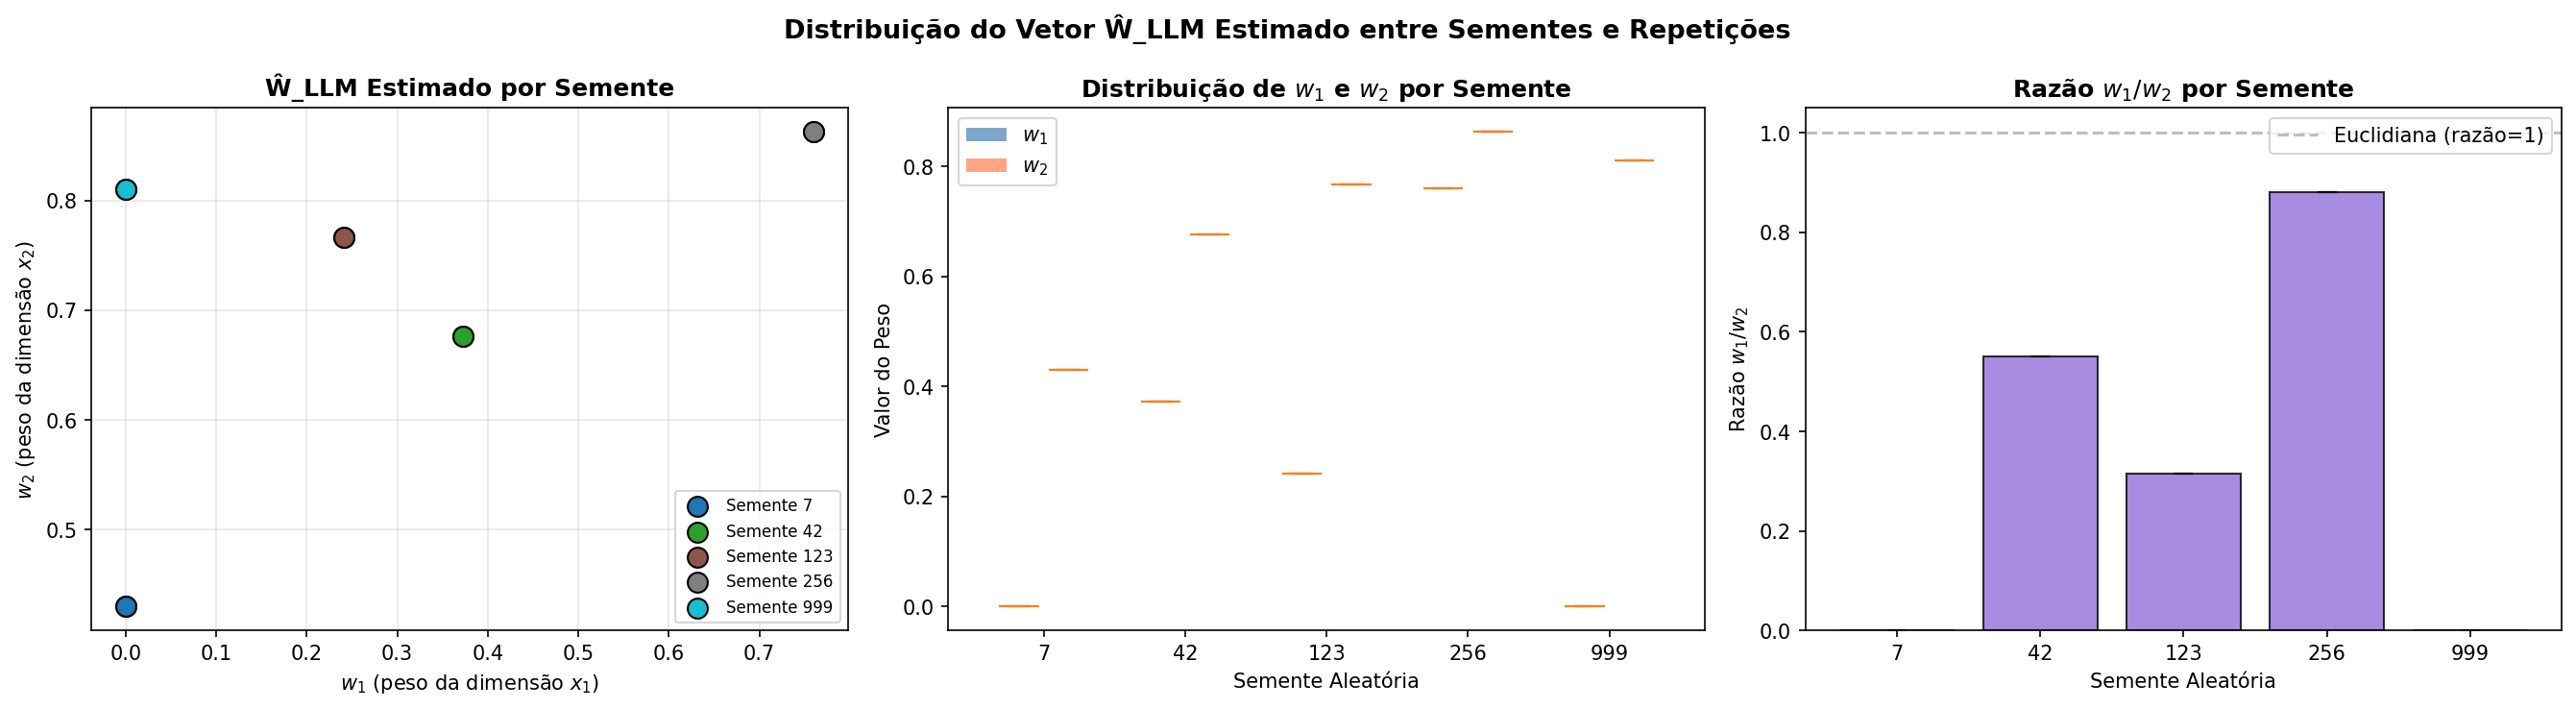
\includegraphics[width=0.78\textwidth]{10_w_distribution.png}
\end{center}
\vspace{-0.2cm}
\small Pesos aprendidos s\~ao \textbf{consistentes em dire\c{c}\~ao}: $w_1 > w_0$ em todas as 5 seeds (raz\~ao $\approx 0.26$--$0.31$). O LLM sistematicamente pesa mais a feature $x_2$.
\end{frame}

% ============================================================
\begin{frame}{Fase A: Erros da M\'etrica vs.\ LLM (Seed 42)}
\begin{center}
    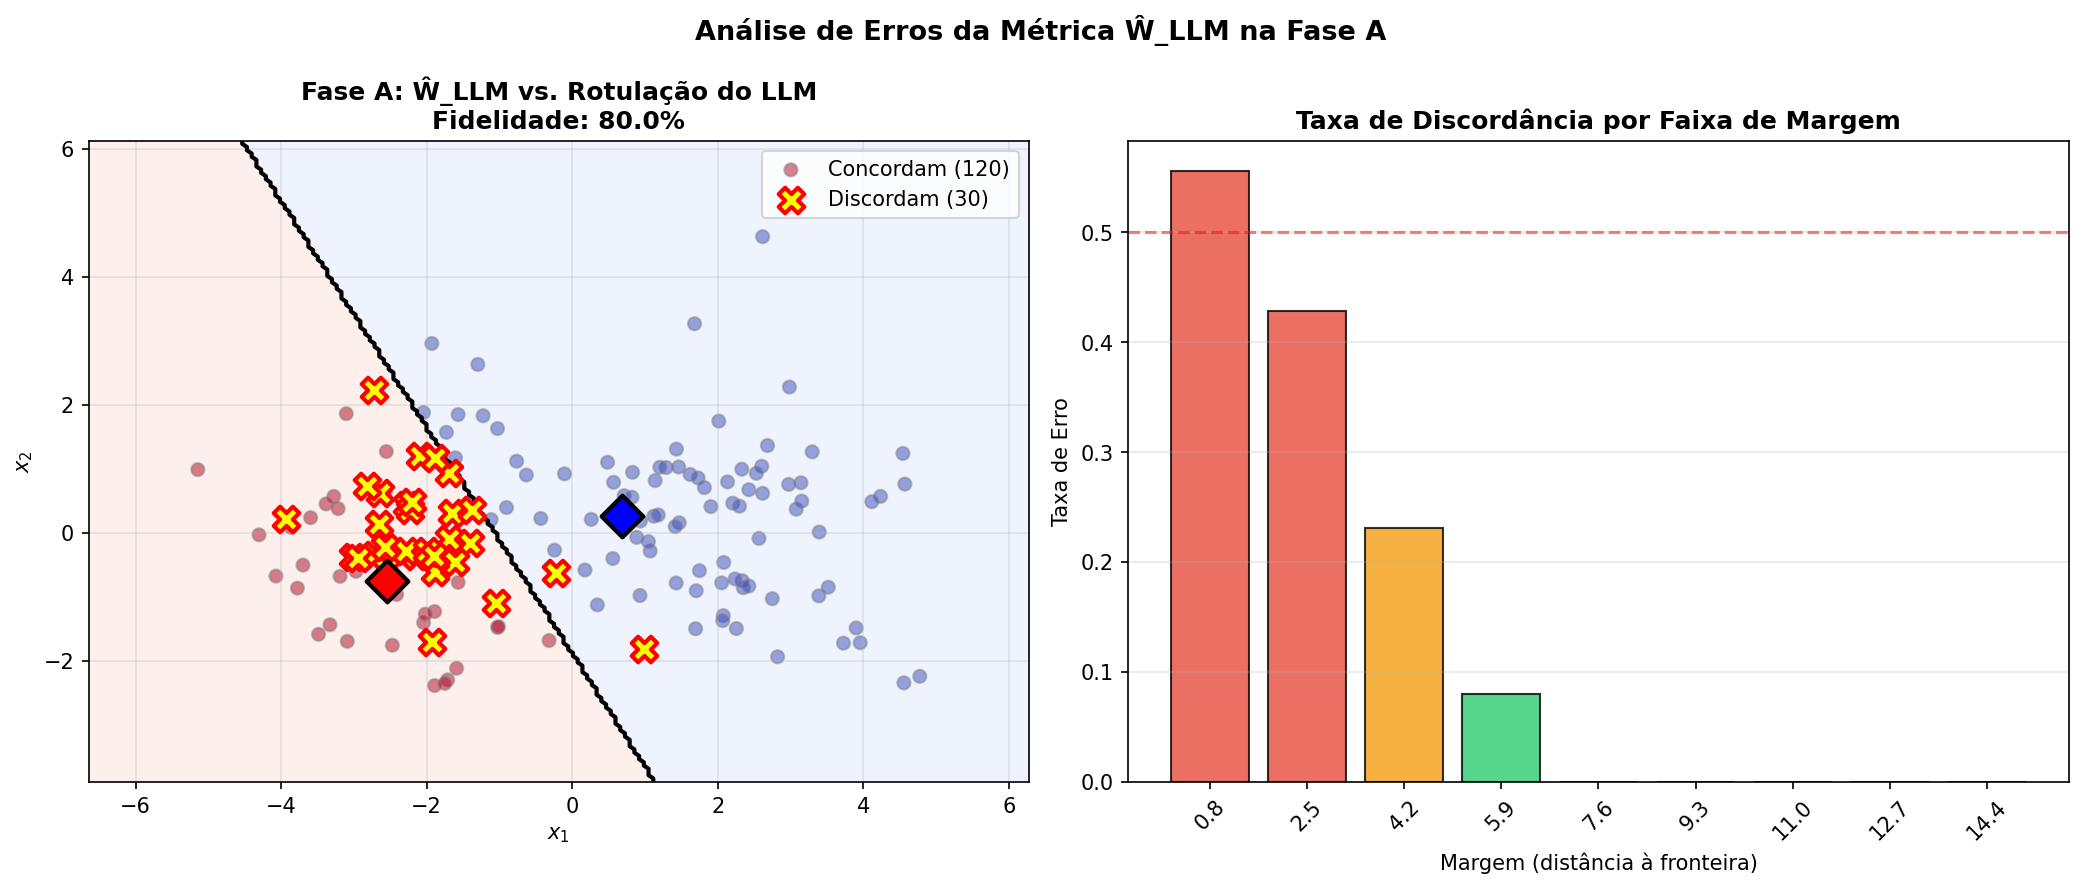
\includegraphics[width=0.72\textwidth]{11_metric_errors_phase_a_seed42.png}
\end{center}
\vspace{-0.2cm}
\small Pontos onde a m\'etrica $\hat{W}_{LLM}$ discorda do LLM. Erros concentram-se pr\'oximos \`a fronteira de decis\~ao --- regi\~ao de maior ambiguidade.
\end{frame}

% ============================================================
\begin{frame}{Fase A: Erros da M\'etrica vs.\ LLM (Seed 256)}
\begin{center}
    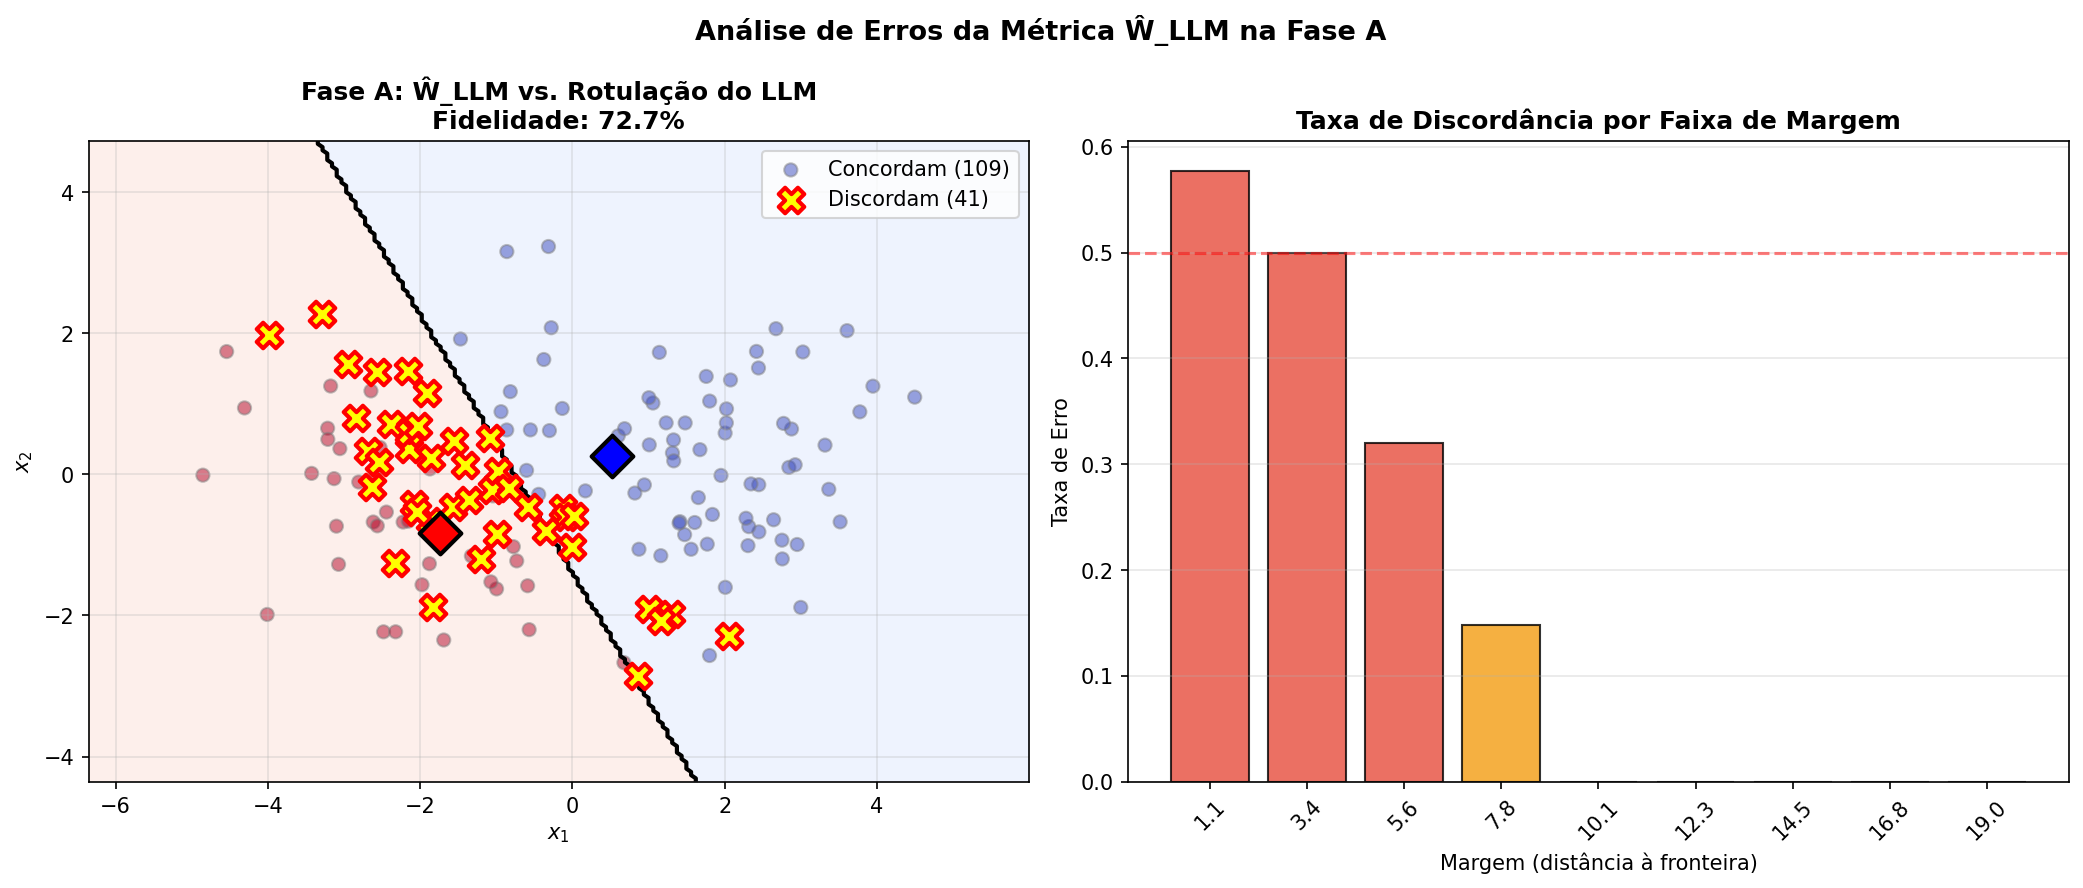
\includegraphics[width=0.72\textwidth]{11_metric_errors_phase_a_seed256.png}
\end{center}
\vspace{-0.2cm}
\small Seed 256 apresenta desempenho superior (+5--7\%) consistentemente. Padr\~ao de erros similar: concentrados na fronteira.
\end{frame}

% ============================================================
\begin{frame}{Fases B/C: Consist\^encia da M\'etrica Transferida}
\begin{center}
    
\includegraphics[width=0.82\textwidth]{02_consistency_extended.png}
\end{center}
\vspace{-0.2cm}
\small \textbf{Problema B:} consist\^encia m\'edia 75.8\% ($\kappa = 0.53$ com 10-shot).
\textbf{Problema C:} 78.5\% ($\kappa = 0.60$). Consist\^encia \textbf{moderada} --- H1 parcialmente confirmada.
\end{frame}

% ============================================================
\begin{frame}{Efeito de Nomes de Classes na Consist\^encia}
\begin{center}
    
\includegraphics[width=0.82\textwidth]{03_class_names_effect.png}
\end{center}
\vspace{-0.2cm}
\small Vi\'es sem\^antico significativo: ``Azul/Vermelho'' atinge 89.7\% vs.\ ``0/1'' com 62.7\%. Nomes semanticamente ricos melhoram consist\^encia em at\'e \textbf{27 pontos percentuais}.
\end{frame}

% ============================================================
\begin{frame}{Vi\'es de Ordem das Classes}
\begin{center}
    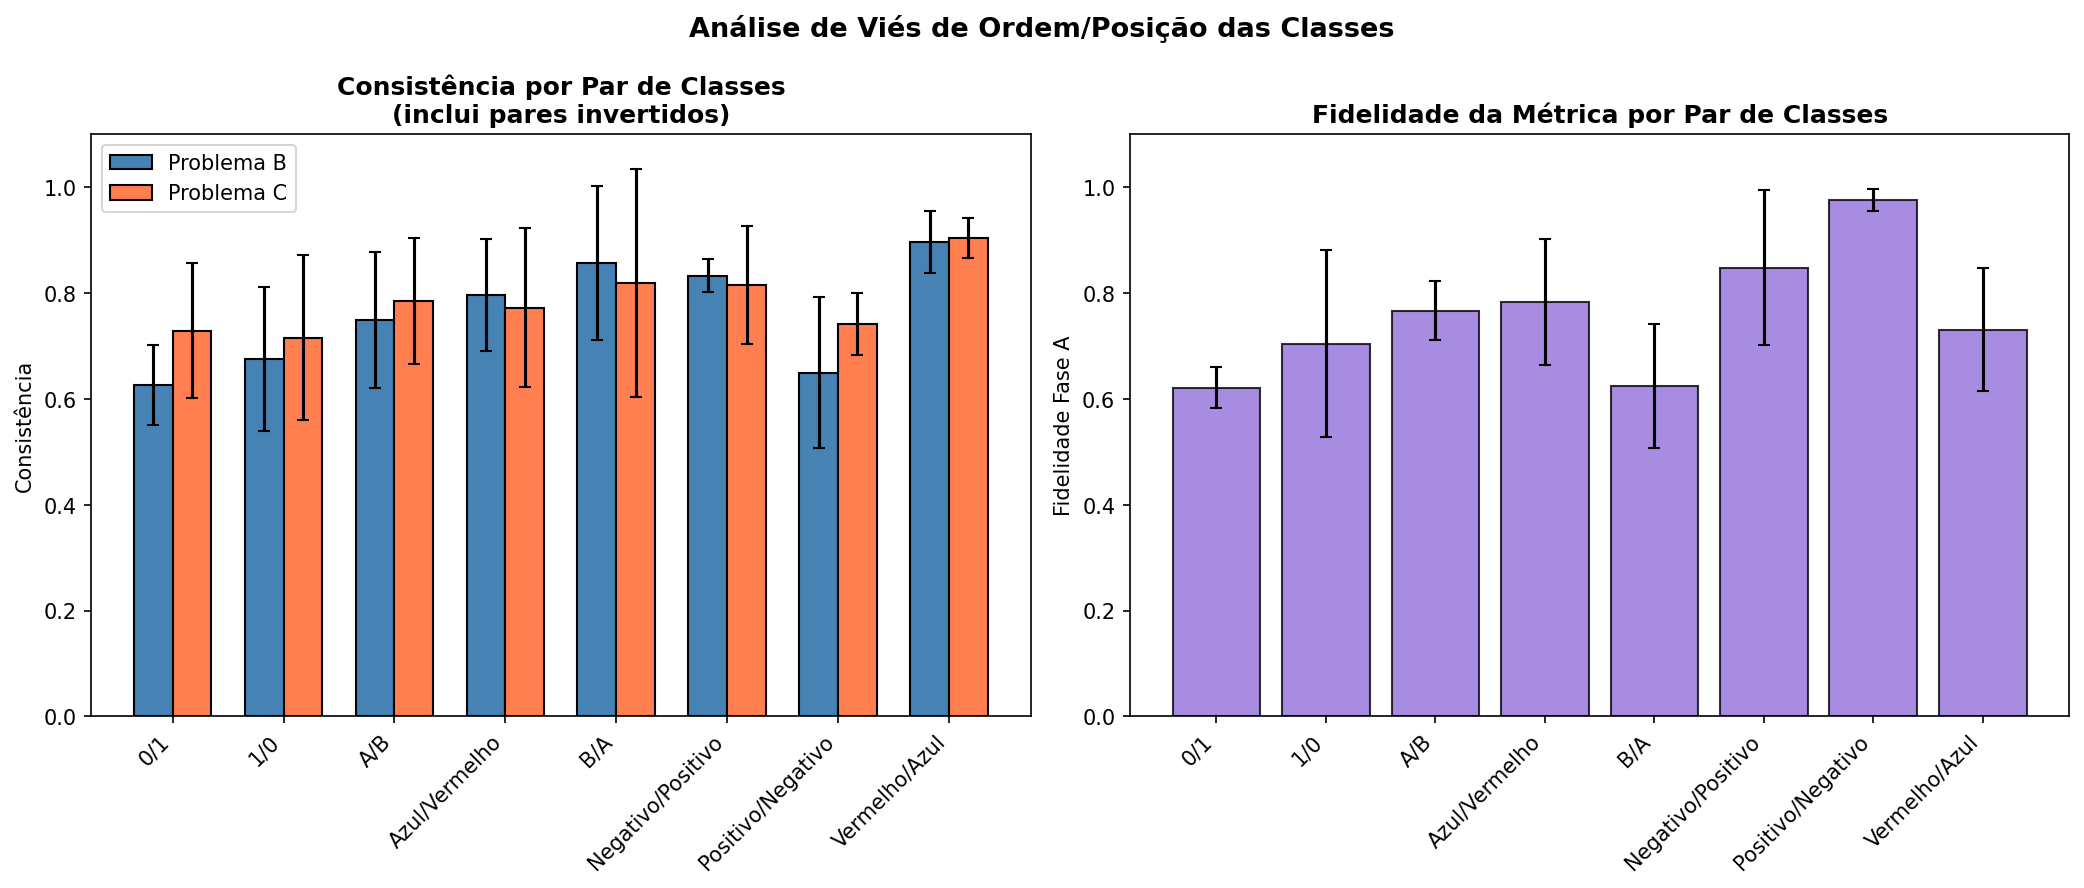
\includegraphics[width=0.82\textwidth]{15_class_order_bias.png}
\end{center}
\vspace{-0.2cm}
\small Inverter a ordem (``A ou B'' $\to$ ``B ou A'') altera resultados em at\'e 20\%. O LLM \'e sens\'ivel \`a posi\c{c}\~ao das classes no prompt --- evid\^encia de vi\'es posicional.
\end{frame}

% ============================================================
\begin{frame}{Robustez entre Seeds (5 Sementes)}
\begin{center}
    
\includegraphics[width=0.82\textwidth]{05_seed_comparison.png}
\end{center}
\vspace{-0.2cm}
\small \textbf{H5 confirmada com ressalvas:} dire\c{c}\~ao de $\hat{W}_{LLM}$ \'e est\'avel ($w_1 > w_0$ em 100\% dos casos), mas magnitude varia. Seed 256 sistematicamente superior.
\end{frame}

% ============================================================
\begin{frame}{Fase D: Problema D com Fronteira do Expert}
\begin{center}
    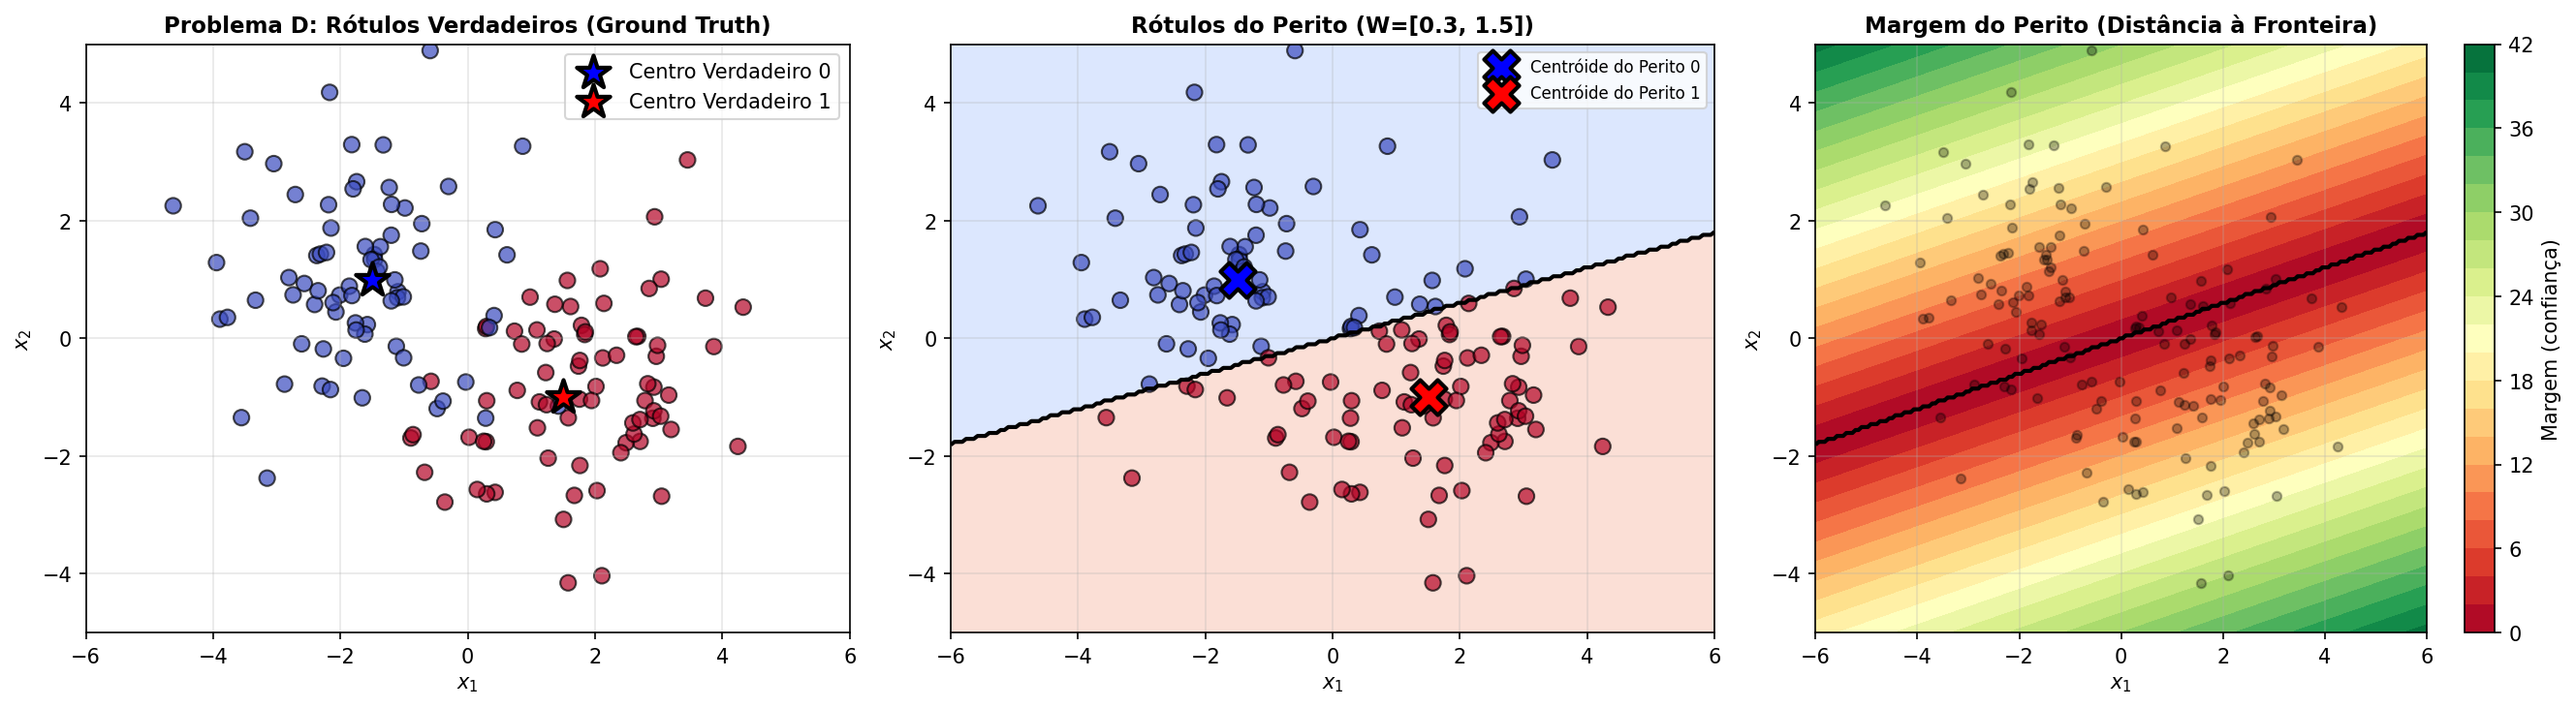
\includegraphics[width=0.72\textwidth]{06_problem_d_expert.png}
\end{center}
\vspace{-0.2cm}
\small Problema D (150 amostras) com fronteira de decis\~ao do expert $W = [0.3, 1.5]$. O expert enfatiza $x_2$ (5$\times$ mais que $x_1$).
\end{frame}

% ============================================================
\begin{frame}{Fase D: Estrat\'egias de Sele\c{c}\~ao de Exemplos}
\begin{center}
    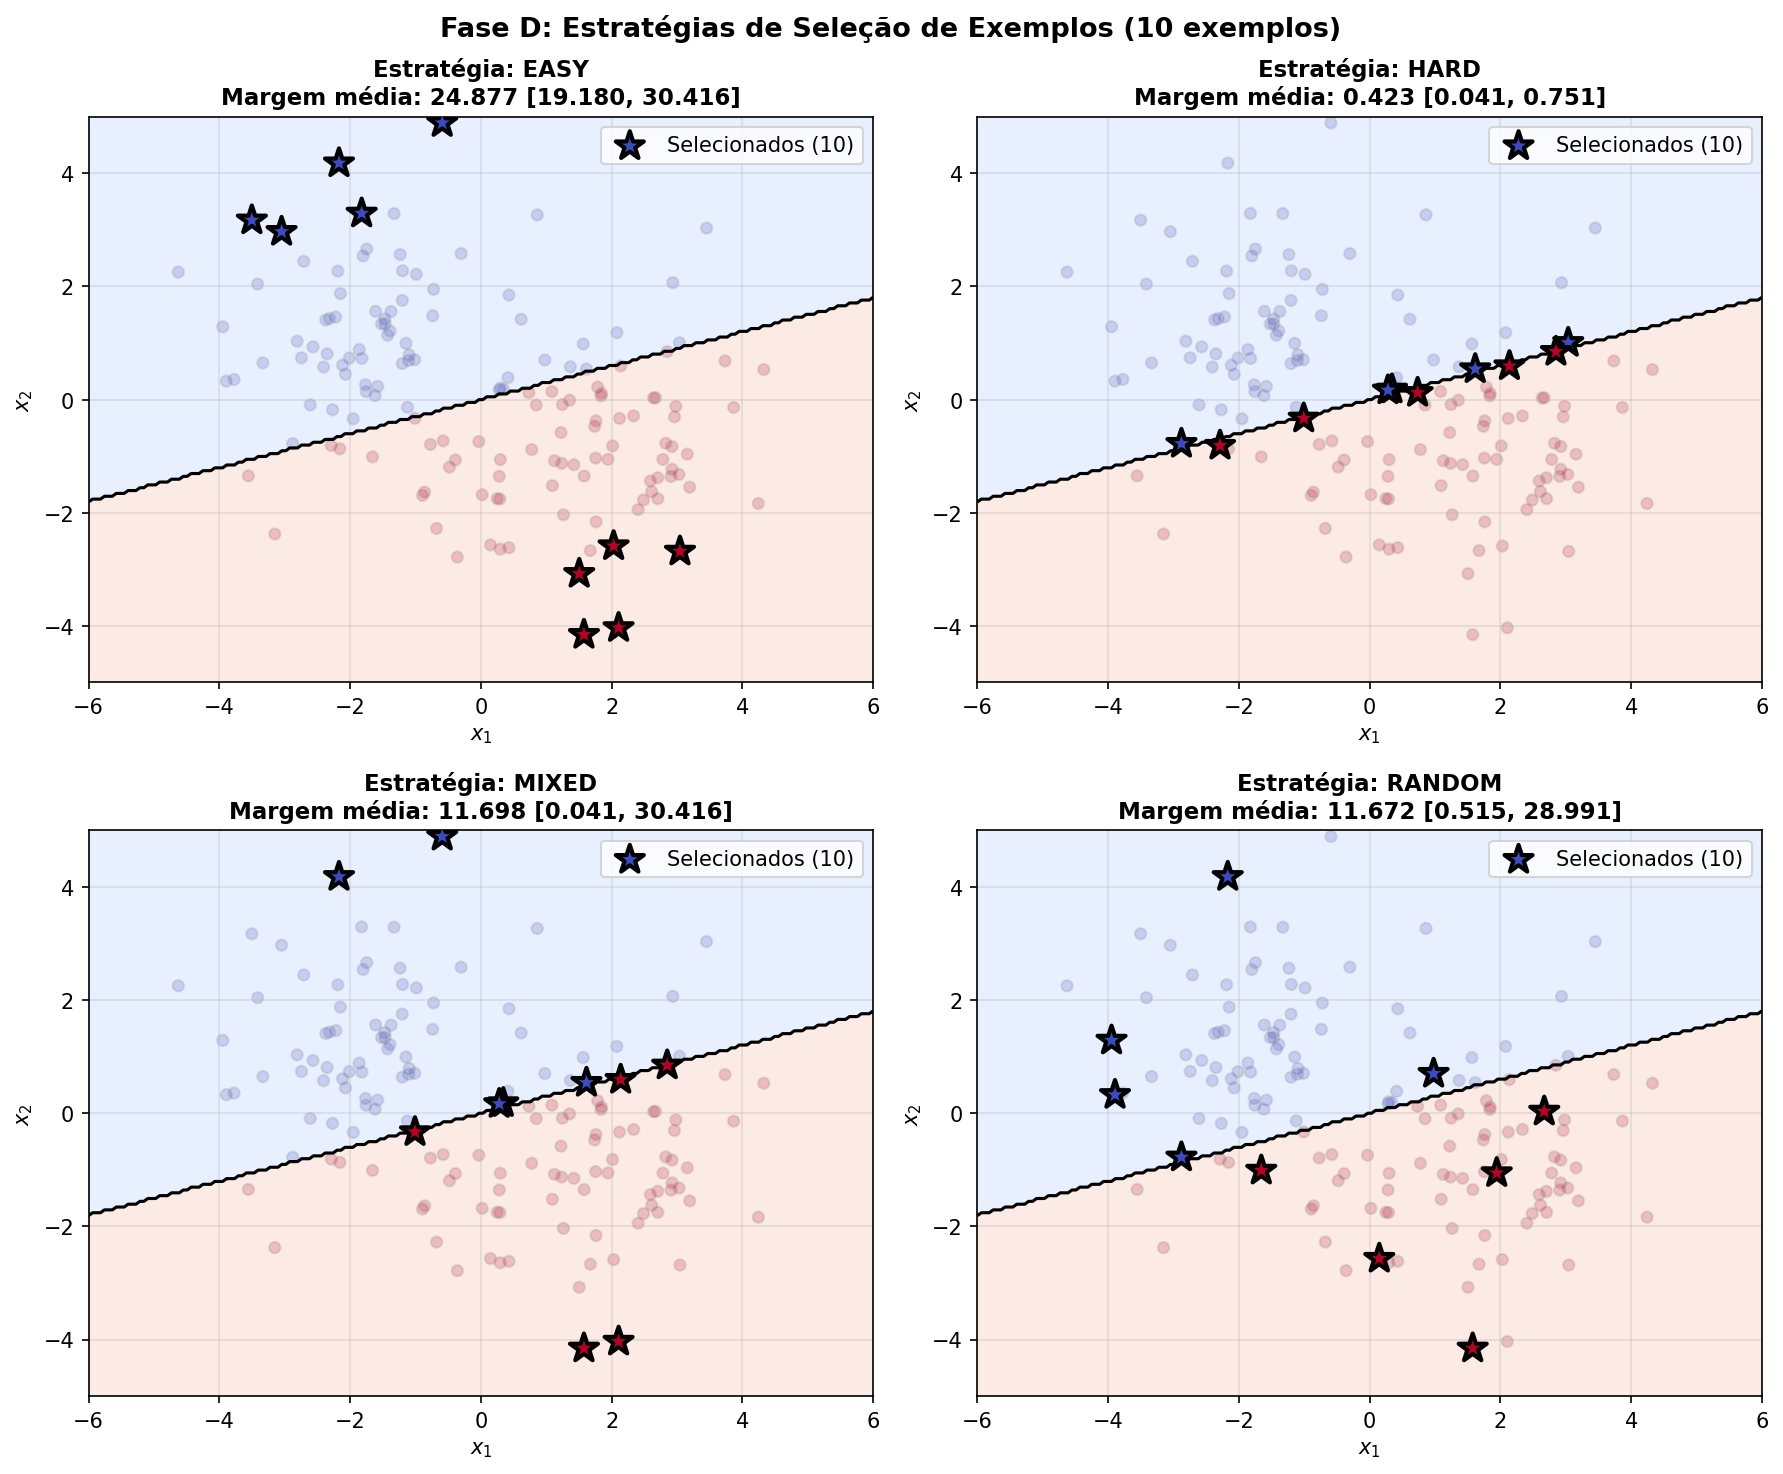
\includegraphics[width=0.82\textwidth]{07_phase_d_example_strategies.png}
\end{center}
\vspace{-0.2cm}
\small Distribui\c{c}\~ao espacial dos exemplos selecionados por cada estrat\'egia. \textbf{Hard:} pr\'oximos \`a fronteira. \textbf{Easy:} longe da fronteira. \textbf{Mixed:} 50\%/50\%. \textbf{Random:} uniforme.
\end{frame}

% ============================================================
\begin{frame}{Fase D: Curva de Aprendizado}
\begin{center}
    
\includegraphics[width=0.82\textwidth]{08_phase_d_learning_curve.png}
\end{center}
\vspace{-0.2cm}
\small \textbf{H3 confirmada:} salto de 56.1\% (zero-shot) para 92.7\% (20-shot random). \textbf{H4 parcialmente refutada:} hard examples prejudicam com poucos exemplos (49.5\% com 3-shot) --- random \'e a melhor estrat\'egia geral.
\end{frame}

% ============================================================
\begin{frame}{Fase D: Compara\c{c}\~ao de Estrat\'egias}
\begin{center}
    
\includegraphics[width=0.82\textwidth]{09_phase_d_strategy_comparison.png}
\end{center}
\vspace{-0.2cm}
\small Compara\c{c}\~ao multi-m\'etrica (acur\'acia, Kappa, F1). \textbf{Random} domina em todos os n\'iveis de few-shot. \textbf{Easy} \'e melhor que hard com poucos exemplos. \textbf{Mixed} converge com random a partir de 10-shot.
\end{frame}

% ============================================================
\begin{frame}{Experimento de Dilui\c{c}\~ao}
\begin{center}
    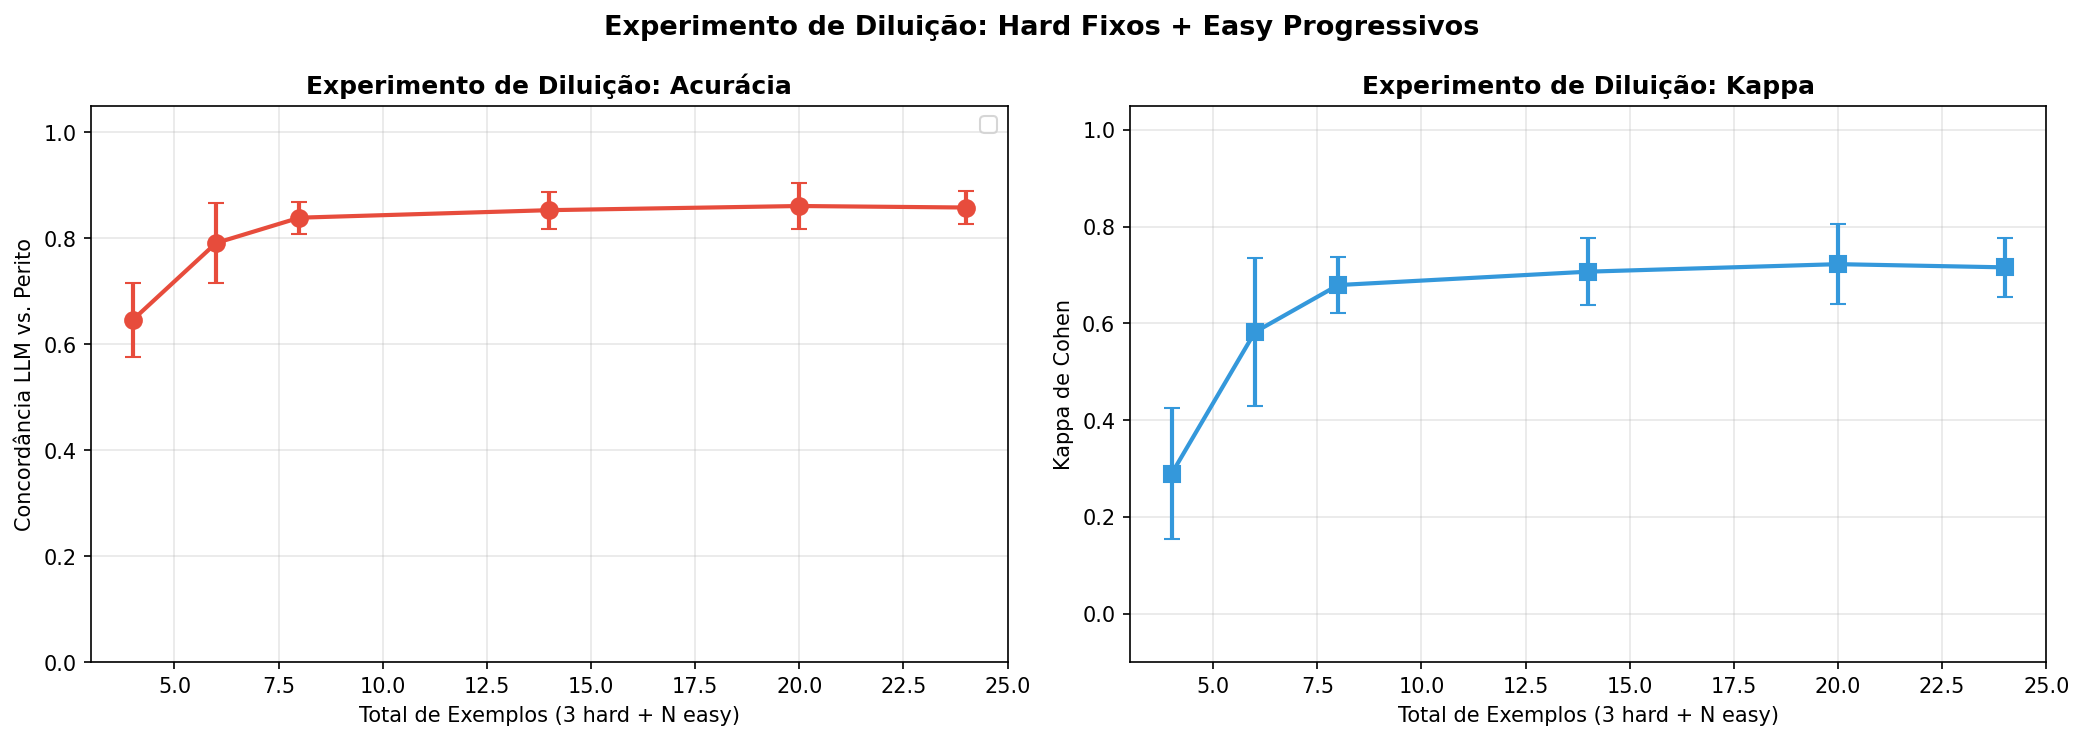
\includegraphics[width=0.82\textwidth]{12_dilution_experiment.png}
\end{center}
\vspace{-0.2cm}
\small 4 exemplos hard fixos + easy progressivos. \textbf{N\~ao h\'a efeito de dilui\c{c}\~ao negativo}: adicionar easy s\'o melhora (57.5\% $\to$ 87.2\%). Retornos decrescentes ap\'os 14 exemplos totais (4 hard + 10 easy).
\end{frame}

% ============================================================
\begin{frame}{Proje\c{c}\~ao R3: 2 Features vs.\ 3 Features}
\begin{center}
    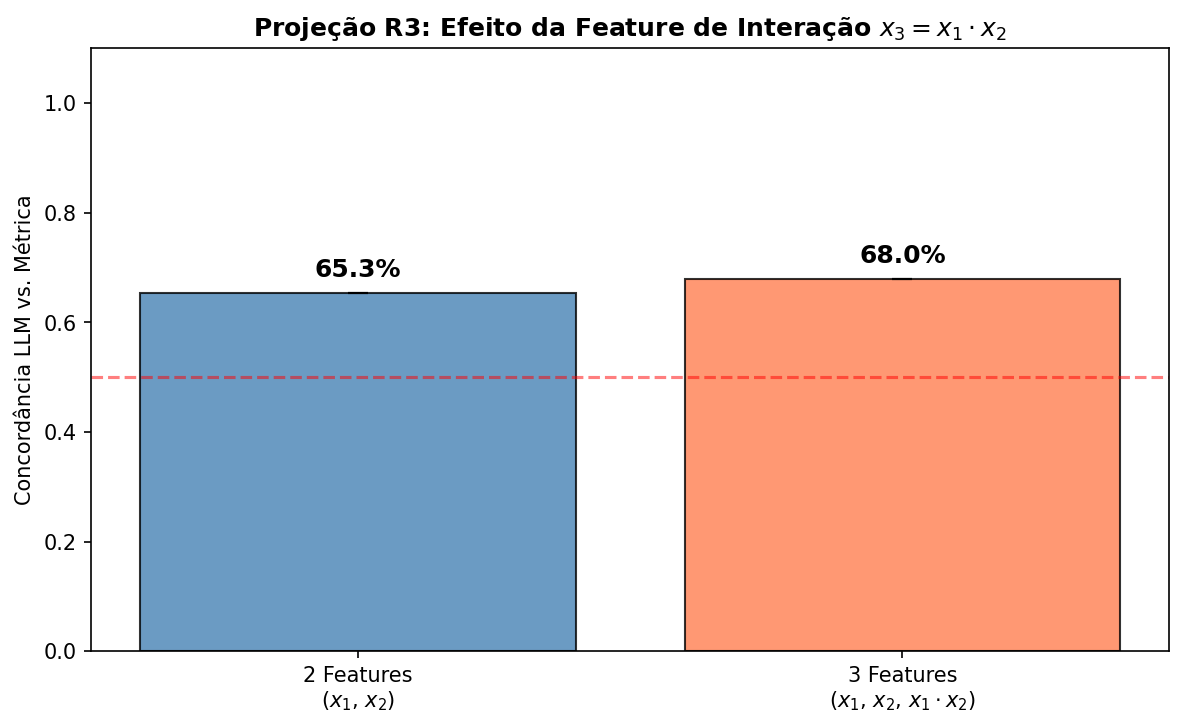
\includegraphics[width=0.82\textwidth]{13_r3_vs_r2.png}
\end{center}
\vspace{-0.2cm}
\small Terceira feature $x_3 = x_1 \cdot x_2$ (kernel quadr\'atico expl\'icito). Compara\c{c}\~ao entre LLM com 2 vs.\ 3 features e m\'etrica com 3 features. Permite capturar intera\c{c}\~oes n\~ao-lineares.
\end{frame}

% ============================================================
\begin{frame}{Compara\c{c}\~ao de Algoritmos: Perceptron vs.\ NNLS}
\begin{center}
    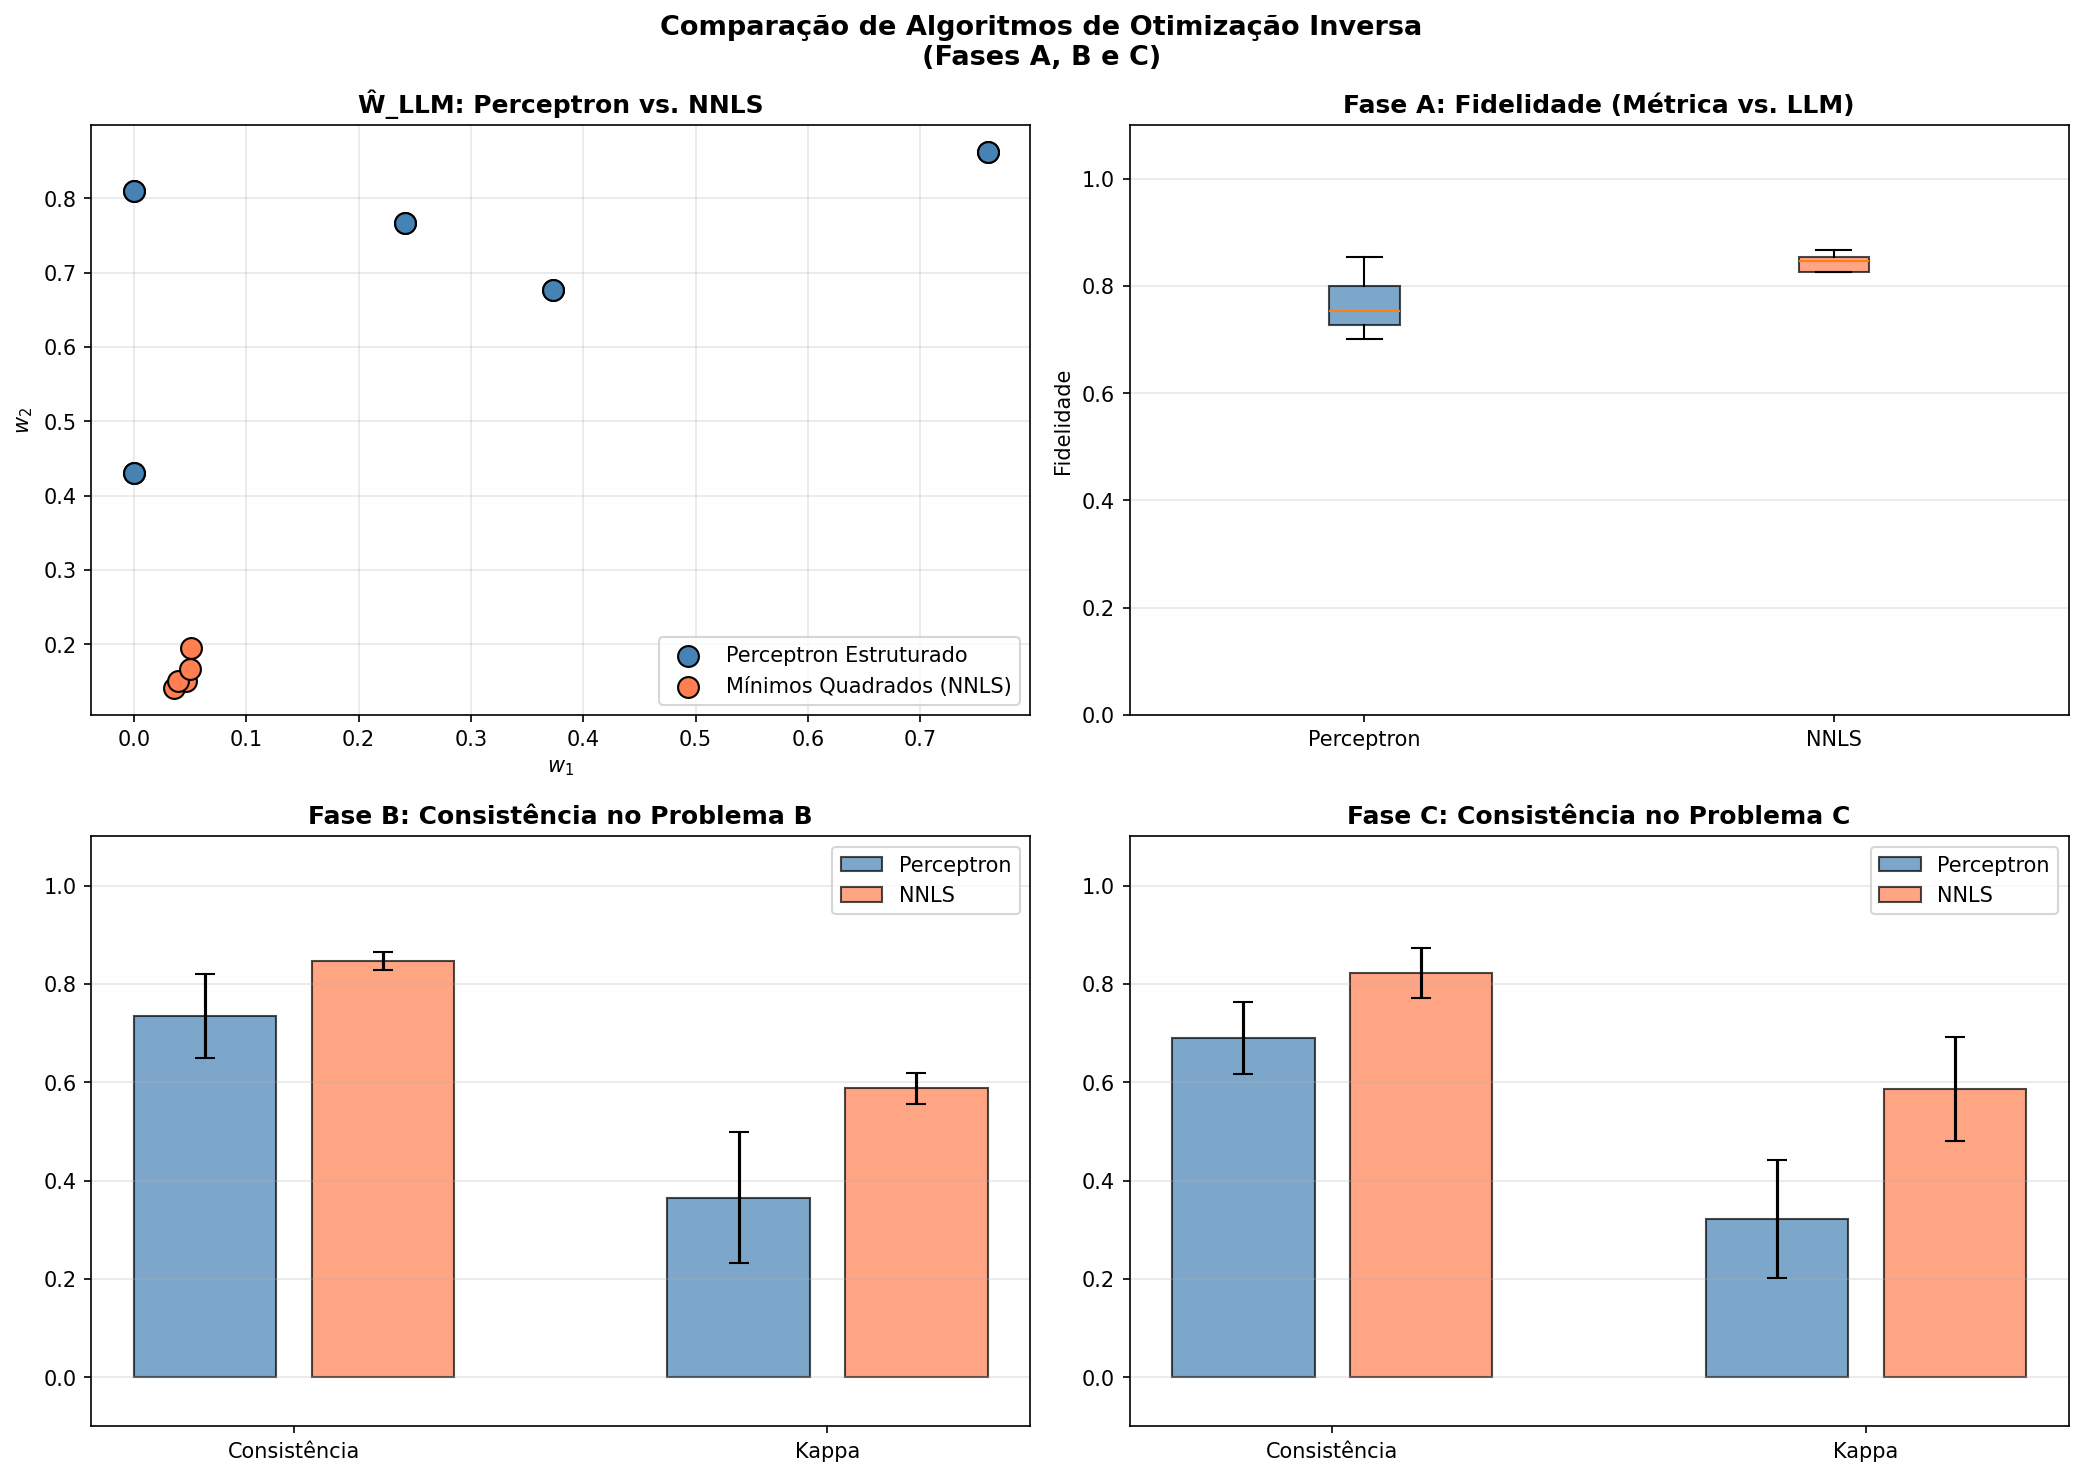
\includegraphics[width=0.82\textwidth]{14_algorithm_comparison.png}
\end{center}
\vspace{-0.2cm}
\small \textbf{NNLS supera Perceptron} em consist\^encia: $\sim$84\% vs.\ $\sim$74\% (+10--15\%). Resultados s\~ao robustos ao m\'etodo de otimiza\c{c}\~ao --- ambos encontram a mesma dire\c{c}\~ao de $\hat{W}$.
\end{frame}

% ============================================================
\begin{frame}{Conclus\~oes: Resultados por Hip\'otese}
\small
\begin{tabular}{@{}lp{7cm}l@{}}
\toprule
\textbf{Hip.} & \textbf{Resultado} & \textbf{Status} \\
\midrule
\textbf{H1} & Consist\^encia 76--79\%, $\kappa \approx 0.53$--$0.60$. $\hat{W}_{LLM}$ est\'avel em dire\c{c}\~ao, mas sens\'ivel a nomes de classes. & \textcolor{orange}{Parcial} \\[4pt]
\textbf{H2} & Few-shot melhora consist\^encia: +10.6\% no Problema C (69\% $\to$ 79.6\%). & \textcolor{green!60!black}{Confirmada} \\[4pt]
\textbf{H3} & LLM aprende expert: 56.1\% $\to$ 92.7\% com 20-shot. Funciona para 3 experts distintos. & \textcolor{green!60!black}{Confirmada} \\[4pt]
\textbf{H4} & Hard examples \textbf{prejudicam} com poucos exemplos (49.5\% vs.\ 84.2\% easy). Random \'e melhor estrat\'egia. & \textcolor{red!70!black}{Refutada} \\[4pt]
\textbf{H5} & Dire\c{c}\~ao de $\hat{W}$ reproduz\'ivel (100\% $w_1 > w_0$). Vari\^ancia em magnitude. & \textcolor{green!60!black}{Confirmada} \\
\bottomrule
\end{tabular}
\end{frame}

% ============================================================
\begin{frame}{Conclus\~oes: Principais Contribui\c{c}\~oes}
\begin{enumerate}
    \item \textbf{O LLM tem crit\'erio decis\'orio moderadamente est\'avel} --- a m\'etrica $\hat{W}_{LLM}$ captura consist\^encia de 76--79\%, com pesos reproduz\'iveis entre seeds

    \vspace{0.2cm}
    \item \textbf{O LLM aprende eficientemente de um expert} --- resultado mais forte: acur\'acia de 92.7\% com 20 exemplos (Fase D)

    \vspace{0.2cm}
    \item \textbf{Exemplos hard n\~ao s\~ao superiores isoladamente} --- a diversidade (random/mixed) \'e mais importante que a dificuldade dos exemplos

    \vspace{0.2cm}
    \item \textbf{Vi\'es sem\^antico \'e significativo} --- nomes de classes e ordem no prompt alteram consist\^encia em at\'e 27 p.p.

    \vspace{0.2cm}
    \item \textbf{Resultados robustos ao algoritmo} --- NNLS e Perceptron convergem na mesma dire\c{c}\~ao de $\hat{W}$
\end{enumerate}
\end{frame}

% ============================================================
\begin{frame}{Pr\'oximos Passos}
\begin{itemize}
    \item Expandir para \textbf{3D com 3 centr\'oides} (tipo Iris) --- valida\c{c}\~ao em maior dimensionalidade
    \item Investigar \textbf{melhorias na fidelidade da Fase A} ($\sim$85\% $\to$ alvo $> 90\%$)
    \item Testar com \textbf{outros LLMs} (Claude, Gemini) para generalidade
    \item Implementar \textbf{algoritmos cl\'assicos de otimiza\c{c}\~ao inversa} (Ahuja \& Orlin)
    \item Explorar \textbf{dados reais} (datasets de refer\^encia)
\end{itemize}

\vspace{0.5cm}
\begin{center}
\Large\textbf{Obrigado!}
\end{center}
\end{frame}

\end{document}
